%
% $Header$
%

\documentclass[11pt]{article}

%\usepackage[dvips]{changebar}

\usepackage{subfigure}
\usepackage{fullpage}
\usepackage{setspace}         % XXX: enabling this may break the compilation
\usepackage{times}
\usepackage{latexsym}
\usepackage{psfig}
\usepackage{graphicx}
\usepackage{xspace}
\usepackage{color}
%\usepackage[dvipdf]{graphics}
%\usepackage[dvips]{graphicx}
%\usepackage{xorp}

\definecolor{gray}{rgb}{0.5,0.5,0.5}
\newcommand{\etc}{\emph{etc.}\xspace}
\newcommand{\ie}{\emph{i.e.,}\xspace}
\newcommand{\eg}{\emph{e.g.,}\xspace}
%\newcommand{\comment}[1]{{\color{gray}[\textsf{#1}]}}
\newcommand{\comment}[1]{}

% Changebar stuff
% \newenvironment{colorcode}{\color{blue}}{}
% \renewcommand{\cbstart}{\begin{colorcode}}
% \renewcommand{\cbend}{\end{colorcode}}

% \pagestyle{empty}

\begin{document}

\title{Using SNMP to manage XORP \\
\vspace{1ex}
Version 0.1}
\author{ XORP Project					\\
	 International Computer Science Institute	\\
	 Berkeley, CA 94704, USA			\\
	 {\it feedback@xorp.org}
}
\date{March 14, 2003}

\maketitle

\thispagestyle{empty}


%%%%%%%%%%%%%%%%%%%%%%%%%%%%%%%%%%%%%%%%%%%%%%%%%%%%%%%%%%%%%%%%%%%%%%%
\section{Introduction}

This document presents the architecture used to allow access to XORP's 
management information via SNMP.  The SNMP standards define the protocol
used to communicate between SNMP managers and agents, as well as the structure
of the management information being accessed (MIB).  This document describes how that
information is made accessible to the SNMP agent, how it is decomposed in 
separate MIB modules, and how those modules are loaded/unloaded at runtime.
The document concludes with a list of guidelines to assist protocol implementers
in writing their own MIB modules for XORP.

%%%%%%%%%%%%%%%%%%%%%%%%%%%%%%%%%%%%%%%%%%%
\section{The SNMP agent}

XORP uses the extensible SNMP agent included in the Net-SNMP package \cite{net-snmp}.  
Net-SNMP provides tools and libraries supporting the Simple Network Management
Protocol.  The package is comprised of an extensible agent, an SNMP library and a
set of command line tools to communicate with SNMP agents and managers. 

Management information is viewed as a collection of managed objects, residing in
a virtual information store, termed the Management Information Base (MIB).  All
managed objects in the MIB are arranged in a hierarchical or tree structure.
Collections of related objects are defined in MIB modules.  These modules are
written in the SNMP data definition language, a subset of Abstract Syntax
Notation One (ASN.1).  New MIB modules that extend the Internet-standard MIB are
continuously being defined by various IETF working groups.  

In the context of this document, we'll extend the term MIB module to include the
part of the code that instantiates the objects declared in the MIB definition
file.  Thus a MIB module consists of:

\begin{description}
    \item[MIB module definition file] This file is written in ASN.1 language, and is
typically published as an RFC.
    \item[MIB module source code] One or more source files that implement the data
access routines that allow the SNMP agent to read or modify XORP's configuration settings. 
\end{description} 






%%%%%%%%%%%%%%%%%%%%%%%%%%%%%%%%%%%%%%%%%%%%%%%%%%%%%%%%%%%%%%%%%%%%%%%
\section{MIB module implementation}
\label{sec:mib_module_implementation}

One of the guiding principles in XORP design is extensibility.  Protocols are
implemented as independent Unix processes that may come and go.  Each protocol
will have one or more associated MIB modules, so those modules should be made
available to the agent without requiring recompilation.  
As explained before, a MIB module contains the code that can access the
management information described in a section of the MIB tree.  Making MIB
modules accessible to the SNMP agent is commonly termed as ''extending the agent''.

Net-SNMP provides three ways to extend the agent:  scripts, dynamically loaded
libraries and sub-agents.


%%%%%%%%%%%%%%%%%%%%%%%%%%%%%%%%%%%%%%%%%%%%%%%%%%%%%%%%%%%%%%%%%%%%%%%
\subsection{Scripts}

Net-SNMP allows runtime agent extension by means of PERL scripts.  In order to
use XORP's IPC libraries to communicate to XORP processes, MIB modules must be
written in C++.  So this alternative will not be used.

%%%%%%%%%%%%%%%%%%%%%%%%%%%%%%%%%%%%%%%%%%%%%%%%%%%%%%%%%%%%%%%%%%%%%%%
\subsection{Dynamically loaded libraries}
Net-SNMP allows the use of dynamically loaded libraries (\ie shared objects).
The libraries must be located in a path accessible to the agent, and are
loaded/unloaded by issuing a set of SNMP commands.  If the SNMP agent was
started with the dynamic library support option, it does not even need to be
restarted:  loading the library will make the new MIB module immediately
accessible.
All SNMP commands relate to one or more Object Identifiers (OIDs) in the MIB
tree.  The information required to load/unload shared libraries (library name, 
path name and load/unload command) is stored under the non Internet-standard branch 
(enterprise-specific) of the MIB tree.
 
Libraries written for the main SNMP agent can also be loaded by an SNMP
sub-agent that communicates with the master agent via the AgentX protocol (see
next subsection).  This has the benefit that time invested in writing MIB modules in this format
will not be wasted if AgentX is to be used for certain protocols in the project. 

%%%%%%%%%%%%%%%%%%%%%%%%%%%%%%%%%%%%%%%%%%%
\subsection{AgentX subagent}

The need of extending SNMP agents at run-time has led vendors to develop a variety of
''extensible agents''.  The AgentX standard \cite{AgentX} is being developed to allow
interoperation of the different solutions.  Within the AgentX framework, an SNMP
agent is defined to consist of:

\begin{itemize}
\item a single processing entity called the master agent, which sends
      and receives SNMP protocol messages in an agent role (as
      specified by the SNMP framework documents) but typically has
      little or no direct access to management information.

\item zero or more processing entities called subagents, which are
      "shielded" from the SNMP protocol messages processed by the
      master agent, but which have access to management information.
\end{itemize}

The master and subagent entities communicate via AgentX protocol messages, which
can use either a network transport mechanism (\eg TCP), or a ''local'' mechanism
(\eg shared memory, named pipes).  Since the AgentX protocol specifies no
security (\ie all sessions are accepted), transport layer security should be
used in the former case.


%%%%%%%%%%%%%%%%%%%%%%%%%%%%%%%%%%%%%%%%%%%
\section{Communicating with XORP}

MIB modules will use XORP's IPC library \cite{xorp:xrl}.  Each MIB module has the
responsibility to pull the relevant management information from the appropriate
process (\eg BGP MIB data from BGP process).  For that effect, the MIB module
must implement the XRL Interface supported by the XRL targets it needs to
communicate to (see \cite{xorp:xrl_interfaces} for details on how to implement
XRL Interface Client classes).  MIB modules, though, MUST not modify any
configuration settings by accessing the process directly.  The current state of
configuration is maintained by the router manager process, so bypassing it would
cause the real and the recorded configurations to be out of sync.  Instead,
configuration changes should be requested to the router manager via
configuration commands, that is, XRLs such as the ones appearing in the template
files (see /xorp/etc/templates/*.tp).

The following diagram illustrates the architecture of MIB modules.
\begin{figure}
  \begin{center}
    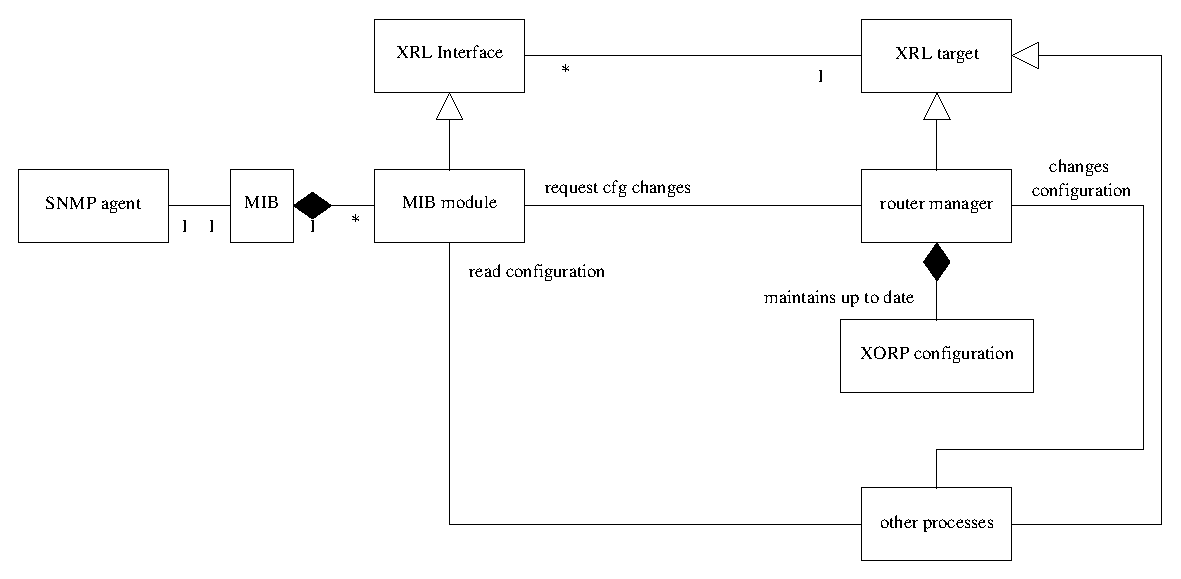
\includegraphics[width=1\textwidth]{figs/snmp_fig1}
  \end{center}
  \caption{Class diagram showing MIB modules interdependencies}
  \label{fig:mib-class-diag}
\end{figure}


%%%%%%%%%%%%%%%%%%%%%%%%%%%%%%%%%%%%%%%%%%%
\section{A reference implementation of a MIB module}

To be continued...


%%%%%%%%%%%%%%%%%%%%%%%%%%%%%%%%%%%%%%%%%%%%%%%%%%%%%%%%%%%%%%%%%%%%%%%
%     APPENDIX
%%%%%%%%%%%%%%%%%%%%%%%%%%%%%%%%%%%%%%%%%%%%%%%%%%%%%%%%%%%%%%%%%%%%%%%
\appendix
\section{Modification History}

\begin{itemize}

  \item March 14, 2003: Created.

\end{itemize}

%%%%%%%%%%%%%%%%%%%%%%%%%%%%%%%%%%%%%%%%%%%%%%%%%%%%%%%%%%%%%%%%%%%%%%%
%     BIBLIOGRAPHY
%%%%%%%%%%%%%%%%%%%%%%%%%%%%%%%%%%%%%%%%%%%%%%%%%%%%%%%%%%%%%%%%%%%%%%%
\bibliography{../tex/xorp}
\bibliographystyle{plain}

%%%%%%%%%%%%%%%%%%%%%%%%%%%%%%%%%%%%%%%%%%%%%%%%%%%%%%%%%%%%%%%%%%%%%%%
\end{document}
